\section{Experiments}
We hypothesize that the proposed methods would improve the performance of the MuZero algorithm. We will now perform several experiments to test and ideally validate this hypothesis.

Note that, in artificial intelligence research and reinforcmeent learning in particular, training processes are stochastic, meaning we need to repeat experiments many times to get statistically significant results. Furthermore, the algorithms are often fragile and highly sensitive to hyperparameter changes. Errors in the implementation are sometimes difficult to find or even notice, given that their impact on the algorithm's performance may be minor.

\subsection{Environments}
For our experiments, we choose environments provided by \textit{OpenAI Gym} \cite{gym}, which is a toolkit for developing and comparing reinforcement learning algorithms. It provides us with a simple and easy to use environment interface and a wide range of environments to develop general purpose agents.

More specifically, we choose two environments, namely \textit{CartPole-v1} and \textit{LunarLander-v2}, shown in figure \ref{fig:environments}. These environments are relatively iconic in the reinforcement learning community, and, due to their simplicity, the learning progress and pitfalls can be easily understood by a human.
\begin{figure}[ht]
    \centering
    \begin{subfigure}{0.49\textwidth}
        \raggedleft
        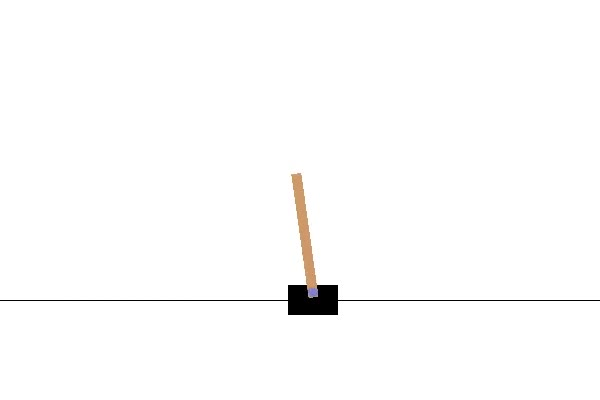
\includegraphics[width=\textwidth]{assets/cartpole.jpg}
    \end{subfigure}
    \begin{subfigure}{0.5\textwidth}
        \raggedright
        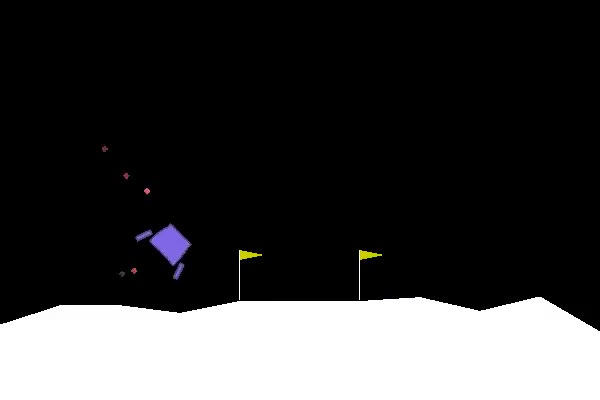
\includegraphics[width=\textwidth]{assets/lunarlander.jpg}
    \end{subfigure}
    \caption{Screenshots of the CartPole-v1 (left) and LunarLander-v2 (right) OpenAI Gym environments.}
    \label{fig:environments}
\end{figure}
A more meaningful benchmark would include significiantly more complex environments, such as Chess and Go, as well as Atari games, as was done for the original MuZero agent. Furthermore, experiments with a robot agents, like a robotic arm grasping for objects, could provide real world applications for the algorithms. Unfortunately, due to MuZero's high computational requirements, we are unable to properly test these environments with various hyperparameters and achieve sufficient statistical significance. The exploration of more demanding environments is therefore left to future work.

In CartPole-v1, the agent controls a cart that can only move horizontally on one axis. Attached to the cart is a pole that starts off relatively upright and can freely spin around the axis perpendicular to the cart's movement. The goal is to balance the pole as long as possible such that it never exceeds $15$ degrees from being vertical. Moving the cart too far to the left or right (i.e. out of bounds) also results in episode termination. Only two actions are available, namely the acceleration in either direction, and a reward of $1$ is given for each survived timestep, up to a maximum of $500$ steps.

The objective in the LunarLander-v2 environment is, as the name suggests, to savely land a lander on the moon's surface. This is done by controlling three thrusters: A main engine, and two orientation thrusters. Various rewards are given to incentivize the agent to pursue this behavior, such as a bonus for approaching the landing pad, and a small negative penalty for using the main engine, encouraging fuel efficiency. Perhaps most notably however, a large negative reward of $-100$ is given for crashing the lander.
\subsection{Setup}
We adopt muzero-general \cite{muzero-general}, an open-source implementation of MuZero that is written in the Python programming language and uses PyTorch for automatic differentiation, as our baselines agent. It is heavily parallelized by employing a worker architecture (see figure \ref{fig:muzero_general}), with each worker being a seperate process that communicates with its peers through message passing. This allows for flexible scaling, even across multiple machines. Worker types include
\begin{itemize}
    \item a \textit{Replay Buffer} worker, responsible for storing game histories as experience for the learning process,
    \item a \textit{Shared Storage} worker, which holds logging information and distributes neural network parameters,
    \item at least one, but potentially many \textit{Self Play} processes, each interacting with its own instance of the environment, collecting experience and filling the replay buffer,
    \item a \textit{Trainer}, which uses stored experience to perform gradient descent on the loss function, thereby improving the model,
    \item the \textit{Reanalyze} worker, responsible for continuously updating outdated search policies and values within the replay buffer and
    \item the main process, which takes logging information from the Shared Storage and outputs it to \textit{TensorBoard}, a tool that allows for live visualization of the training process.
\end{itemize}
Note that the term \textit{self-play} originates from AlphaZero or MuZero agents playing a board game like Chess against themselves to learn strategies without any human influence. Regardless, we use the term even for environments operated by only a single player, such as LunarLander-v2.
\begin{figure}[ht]
    \centering
    \tikzset{%
        cascaded/.style = {%
            general shadow = {%
            shadow scale = 1,
            shadow xshift = -1ex,
            shadow yshift = -1ex,
            draw,
            thick,
            fill = white},
            general shadow = {%
            shadow scale = 1,
            shadow xshift = -.5ex,
            shadow yshift = -.5ex,
            draw,
            thick,
            fill = white},
            fill = white, 
            draw,
            thick,
        }
    }
    \begin{tikzpicture}[every node/.style={inner sep=0.3cm}]
        \node [draw, rectangle] (reanalyze) {Reanalyze};
        \node [draw, rectangle, below = of reanalyze] (replay) {Replay Buffer};
        \node [draw, rectangle, below = 1.5cm of replay] (storage) {Shared Storage};
        \node [draw, rectangle, left = 2.5cm of storage] (trainer) {Trainer};
        \node [draw, rectangle, cascaded, right = 2.5cm of storage] (play) {Self Play};
        \node [draw, rectangle, below = 1.5cm of storage] (tensorboard) {TensorBoard};

        \draw [->] (reanalyze) edge [bend right] node[left] {update game history} (replay);
        \draw [->] (replay) edge [bend right] node[right] {sample game history} (reanalyze);

        \draw [->] (trainer) -- node[below right=-0.2cm] {update priorities} (replay);
        \draw [->] (replay) edge [bend right] node[above left] {get batch} (trainer);
        \draw [->] (trainer) -- node[below] {set weights} (storage);
        \draw [->] (storage) -- node[below] {get weights} (play);
        \draw [->] (play) -- node[above right] {save game history} (replay);

        \draw [->] (storage) -- node[left] {get info} (tensorboard);
    \end{tikzpicture}
    \caption{The parallelized worker structure of muzero-general.}
    \label{fig:muzero_general}
\end{figure}

We modify the source code of muzero-general to include a reconstruction function and the additional loss terms. The readout of the replay buffer must also be tweaked to include not only the observation at timestep $t$, but the $K$ subsequent observations $o_{t+1}, ..., o_{t+K}$ as well, as they are critical for calculating our new loss values.

The neural networks making up each of the three MuZero functions and our new reconstruction function follow a very simple structure in all experiments. They consist of simple two-layered fully connected perceptrons. The first (\textit{hidden}) layer contains 16 neurons in the case of CartPole-v1 and 64 for LunarLander-v2. The number of neurons in the second layer is determined by the desired output dimensionality. For example, the representation function must output an internal state, which, for CartPole-v1, is an eight-dimensional vector. Thus, the second layer is made up of eight neurons.

A variety of different weights are tested for each of the two loss terms in order to gauge their capability of improving performance, both individually and in a union. Furthermore, as a means of showcasing self-supervised learning for MuZero, we pretrain a hybrid agent, that is, an agent using both modifications at the same time, for $5000$ training steps, using only the newly added loss terms, instead of the full loss formula.

Table \ref{tab:hyperparameters} shows the hyperparameters used by all tested model configurations. Based on the muzero-general default parameters, only the number of training steps was reduced to be able to perform additional test runs with the newly freed resources. Note that we are unable to perform a comprehensive hyperparameter search due to technical limitations.
\begin{table}[ht]
    \centering
    \begin{tabular}{|c|l||c|c|}
        \hline
        & & CartPole-v1 & LunarLander-v2 \\
        \hline\hline

        & Training steps & $10000^*$ & $30000^*$ \\
        \cline{2-4}
        & Discount factor ($\gamma$) & 0.997 & 0.999 \\
        \cline{2-4}
        & TD steps ($n$) & 50 & 30 \\
        \cline{2-4}
        & Unroll steps ($K$) & 10 & 10 \\
        \cline{2-4}
        & Internal state dimensions & 8 & 10 \\
        \cline{2-4}
        & MuZero Reanalyze & Enabled & Enabled \\

        \hline

        \multirow{4.1}{*}{\begin{sideways}Losses\end{sideways}} & Optimizer & Adam & Adam \\
        \cline{2-4}
        & Learning rate ($\beta$) & $0.02 \times 0.9^{t \times 0.001}$ & 0.005 \\
        \cline{2-4}
        & Value loss weight & 1.0 & 1.0 \\
        \cline{2-4}
        & L2 regularization weight & $10^{-4}$ & $10^{-4}$ \\

        \hline

        \multirow{3.2}{*}{\begin{sideways}Replay\end{sideways}} & Replay buffer size & 500 & 2000 \\
        \cline{2-4}
        & Prioritization exponent & 0.5 & 0.5 \\
        \cline{2-4}
        & Batch size & 128 & 64 \\

        \hline

        \multirow{7.5}{*}{\begin{sideways}MCTS\end{sideways}} & Simulations & 50 & 50 \\
        \cline{2-4}
        & Dirichlet $\alpha$ & 0.25 & 0.25 \\
        \cline{2-4}
        & Exploration factor & 0.25 & 0.25 \\
        \cline{2-4}
        & pUCT $c_1$ & 1.25 & 1.25 \\
        \cline{2-4}
        & pUCT $c_2$ & 19652 & 19652 \\
        \cline{2-4}
        & Softmax temperature ($T$) & \makecell{
            1.0 if $t<5000$, \\ 0.5 if $5000 \leq t < 7500$, \\ 0.25 if $t \geq 7500$
        } & 0.35 \\

        \hline
    \end{tabular}
    \caption{Hyperparameter selection for all tested agents. Parameters based on the current training step use the variable $t$. Only parameters marked with a $^*$ are different from the muzero-general defaults.}
    \label{tab:hyperparameters}
\end{table}

 Performance is measured by training an agent for a specific amount of training steps and, at various time steps, sampling the total episode reward the agent can achieve.

\subsection{Results}
We show a comparison of the performance of agents with different weights applied to each loss term proposed in this thesis. For our notation, we use $l^g$ and $l^c$ for the reconstruction function and consistency loss modification, respectively. With $\frac{1}{2}l^g$ and $\frac{1}{2}l^g$ we denote that the default loss weight of $1$ for each term has been changed to $\frac{1}{2}$. Finally, we write a plus sign to indicate the combination of both modifications.

The results in Figure \ref{fig:reconstruction_results} show an increase in performance when adding the reconstruction function together with its associated loss term to the MuZero algorithm on all testing environments. Weighting the reconstruction loss term with $\frac{1}{2}$ only has a minor negative impact on the learning process. Note that, in the LunarLander-v2 environment, a penalty reward of $-100$ is given to an agent for crashing the lander. The default MuZero agent was barely able to exceed this threshold, whereas the reconstruction agent achieved positive total rewards.

The consistency loss term agent matched or only very slightly exceeded the performance of MuZero in the CartPole-v1 environment, as can be seen in Figure \ref{fig:consistency_results} (left). However, in the LunarLander-v2 task, the modified agent significantly outperformed MuZero, being almost at the same level as the reconstruction agent. A loss weight of $1$ is also notably better than a loss weight of $\frac{1}{2}$.

An agent using both loss terms simultaneously outperforms MuZero (visible in Figure \ref{fig:hybrid_results}), and even scores marginally better than the reconstruction loss agent, in all environments tested.

When using self-supervised pretraining (see Figure \ref{fig:pretrained_results}), training progresses very rapidly as soon as the goal is introduced. In the LunarLander-v2 environment, a mean total reward of $0$ is reached in roughly half the amount of training steps that are required by the non-pretrained agent. However, at later stages of training, the advantage fades, and, in the case of CartPole-v1, agents using self-supervised pretraining perform significantly worse than agents starting with randomly initialized networks.

The fully trained agents are compared in Table \ref{tab:results_table}. Training took place on NVIDIA GeForce GTX 1080 and NVIDIA GeForce RTX 2080 Ti GPUs. Each experiment required roughly two to three days to complete.

\begin{figure}[H]
    \centering
    \begin{tikzpicture}[yscale=0.7, xscale=0.7,
                        define rgb/.code={\definecolor{mycolor}{RGB}{#1}},
                        rgb color/.style={define rgb={#1},mycolor}]
        \begin{axis}[
            title = CartPole-v1,
            axis lines = left,
            xlabel = Training steps,
            ylabel = Total reward,
            no markers,
            table/col sep = comma,
            legend cell align=left,
            legend pos=south east,
            legend style={draw=none},
            xmin=0,
            xmax=10000,
            grid=major,
        ]
            \addplot[black] table [
                x = training_step,
                y = reward,
            ] {results/default/CartPole-v1/lr0.0.csv};
            \addlegendentry{MuZero};

            \addplot[rgb color={32, 32, 180}] table [
                x = training_step,
                y = reward,
            ] {results/reconstruction/CartPole-v1/lr0.5.csv};
            \addlegendentry{$\frac{1}{2}l^g$};

            \addplot[rgb color={128, 128, 255}] table [
                x = training_step,
                y = reward,
            ] {results/reconstruction/CartPole-v1/lr1.0.csv};
            \addlegendentry{$l^g$};
        \end{axis}
    \end{tikzpicture}
    \begin{tikzpicture}[yscale=0.7, xscale=0.7,
                        define rgb/.code={\definecolor{mycolor}{RGB}{#1}},
                        rgb color/.style={define rgb={#1},mycolor}]
        \begin{axis}[
            title = LunarLander-v2,
            axis lines = left,
            xlabel = Training steps,
            ylabel = Total reward,
            no markers,
            table/col sep = comma,
            legend cell align=left,
            legend pos=south east,
            legend style={draw=none},
            xmin=0,
            xmax=30000,
            grid=major,
        ]
            \addplot[black] table [
                x = training_step,
                y = reward,
            ] {results/default/LunarLander-v2/lr0.0.csv};
            \addlegendentry{MuZero};

            \addplot[rgb color={32, 32, 180}] table [
                x = training_step,
                y = reward,
            ] {results/reconstruction/LunarLander-v2/lr0.5.csv};
            \addlegendentry{$\frac{1}{2}l^g$};

            \addplot[rgb color={128, 128, 255}] table [
                x = training_step,
                y = reward,
            ] {results/reconstruction/LunarLander-v2/lr1.0.csv};
            \addlegendentry{$l^g$};
        \end{axis}
    \end{tikzpicture}
    \caption{Total episode reward comparison of agents using the reconstruction loss term ($l^g$) and the default MuZero agent in the CartPole-v1 and LunarLander-v2 environments, averaged across 32 and 25 runs, respectively.}
    \label{fig:reconstruction_results}
\end{figure}

\begin{figure}[H]
    \centering
    \begin{tikzpicture}[yscale=0.7, xscale=0.7,
                        define rgb/.code={\definecolor{mycolor}{RGB}{#1}},
                        rgb color/.style={define rgb={#1},mycolor}]
        \begin{axis}[
            title = CartPole-v1,
            axis lines = left,
            xlabel = Training steps,
            ylabel = Total reward,
            no markers,
            table/col sep = comma,
            legend cell align=left,
            legend pos=south east,
            legend style={draw=none},
            xmin=0,
            xmax=10000,
            grid=major,
        ]
            \addplot[black] table [
                x = training_step,
                y = reward,
            ] {results/default/CartPole-v1/lr0.0.csv};
            \addlegendentry{MuZero};

            \addplot[rgb color={32, 128, 32}] table [
                x = training_step,
                y = reward,
            ] {results/consistency/CartPole-v1/lr0.5.csv};
            \addlegendentry{$\frac{1}{2}l^c$};

            \addplot[rgb color={0, 255, 0}] table [
                x = training_step,
                y = reward,
            ] {results/consistency/CartPole-v1/lr1.0.csv};
            \addlegendentry{$l^c$};
        \end{axis}
    \end{tikzpicture}
    \begin{tikzpicture}[yscale=0.7, xscale=0.7,
                        define rgb/.code={\definecolor{mycolor}{RGB}{#1}},
                        rgb color/.style={define rgb={#1},mycolor}]
        \begin{axis}[
            title = LunarLander-v2,
            axis lines = left,
            xlabel = Training steps,
            ylabel = Total reward,
            no markers,
            table/col sep = comma,
            legend cell align=left,
            legend pos=south east,
            legend style={draw=none},
            xmin=0,
            xmax=30000,
            grid=major,
        ]
            \addplot[black] table [
                x = training_step,
                y = reward,
            ] {results/default/LunarLander-v2/lr0.0.csv};
            \addlegendentry{MuZero};

            \addplot[rgb color={32, 128, 32}] table [
                x = training_step,
                y = reward,
            ] {results/consistency/LunarLander-v2/lr0.5.csv};
            \addlegendentry{$\frac{1}{2}l^c$};

            \addplot[rgb color={0, 255, 0}] table [
                x = training_step,
                y = reward,
            ] {results/consistency/LunarLander-v2/lr1.0.csv};
            \addlegendentry{$l^c$};
        \end{axis}
    \end{tikzpicture}
    \caption{Total episode reward comparison of agents the consistency loss ($l^c$) and the default MuZero agent in the CartPole-v1 and LunarLander-v2 environments, averaged across 32 and 25 runs, respectively.}
    \label{fig:consistency_results}
\end{figure}

\begin{figure}[H]
    \centering
    \begin{tikzpicture}[yscale=0.7, xscale=0.7,
                        define rgb/.code={\definecolor{mycolor}{RGB}{#1}},
                        rgb color/.style={define rgb={#1},mycolor}]
        \begin{axis}[
            title = CartPole-v1,
            axis lines = left,
            xlabel = Training steps,
            ylabel = Total reward,
            no markers,
            table/col sep = comma,
            legend cell align=left,
            legend pos=south east,
            legend style={draw=none},
            xmin=0,
            xmax=10000,
            grid=major,
        ]
            \addplot[black] table [
                x = training_step,
                y = reward,
            ] {results/default/CartPole-v1/lr0.0.csv};
            \addlegendentry{MuZero};

            \addplot[rgb color={128, 128, 255}] table [
                x = training_step,
                y = reward,
            ] {results/reconstruction/CartPole-v1/lr1.0.csv};
            \addlegendentry{$l^g$};

            \addplot[rgb color={0, 128, 128}] table [
                x = training_step,
                y = reward,
            ] {results/hybrid/CartPole-v1/lr0.5.csv};
            \addlegendentry{$\frac{1}{2}l^g + \frac{1}{2}l^c$};

            \addplot[rgb color={0, 200, 200}] table [
                x = training_step,
                y = reward,
            ] {results/hybrid/CartPole-v1/lr1.0.csv};
            \addlegendentry{$l^g + l^c$};
        \end{axis}
    \end{tikzpicture}
    \begin{tikzpicture}[yscale=0.7, xscale=0.7,
                        define rgb/.code={\definecolor{mycolor}{RGB}{#1}},
                        rgb color/.style={define rgb={#1},mycolor}]
        \begin{axis}[
            title = LunarLander-v2,
            axis lines = left,
            xlabel = Training steps,
            ylabel = Total reward,
            no markers,
            table/col sep = comma,
            legend cell align=left,
            legend pos=south east,
            legend style={draw=none},
            xmin=0,
            xmax=30000,
            grid=major,
        ]
            \addplot[black] table [
                x = training_step,
                y = reward,
            ] {results/default/LunarLander-v2/lr0.0.csv};
            \addlegendentry{MuZero};

            \addplot[rgb color={128, 128, 255}] table [
                x = training_step,
                y = reward,
            ] {results/reconstruction/LunarLander-v2/lr1.0.csv};
            \addlegendentry{$l^g$};

            \addplot[rgb color={0, 128, 128}] table [
                x = training_step,
                y = reward,
            ] {results/hybrid/LunarLander-v2/lr0.5.csv};
            \addlegendentry{$\frac{1}{2}l^g + \frac{1}{2}l^c$};

            \addplot[rgb color={0, 200, 200}] table [
                x = training_step,
                y = reward,
            ] {results/hybrid/LunarLander-v2/lr1.0.csv};
            \addlegendentry{$l^g + l^c$};
        \end{axis}
    \end{tikzpicture}
    \caption{Total episode reward comparison of agents using both the reconstruction function loss ($l^g$) as well as the consistency loss term ($l^c$) simultaneously in the CartPole-v1 and LunarLander-v2 environments, averaged across 32 and 25 runs, respectively.}
    \label{fig:hybrid_results}
\end{figure}

\begin{figure}[H]
    \centering
    \begin{tikzpicture}[yscale=0.7, xscale=0.7,
                        define rgb/.code={\definecolor{mycolor}{RGB}{#1}},
                        rgb color/.style={define rgb={#1},mycolor}]
        \begin{axis}[
            title = CartPole-v1,
            axis lines = left,
            xlabel = Training steps,
            ylabel = Total reward,
            no markers,
            table/col sep = comma,
            legend cell align=left,
            legend pos=south east,
            legend style={draw=none},
            xmin=0,
            xmax=10000,
            grid=major,
        ]
            \addplot[black] table [
                x = training_step,
                y = reward,
            ] {results/default/CartPole-v1/lr0.0.csv};
            \addlegendentry{MuZero};

            \addplot[rgb color={0, 200, 200}] table [
                x = training_step,
                y = reward,
            ] {results/hybrid/CartPole-v1/lr1.0.csv};
            \addlegendentry{$l^g + l^c$};

            \addplot[rgb color={220, 80, 80}] table [
                x = training_step,
                y = reward,
            ] {results/pretrained/CartPole-v1/lr1.0.csv};
            \addlegendentry{$l^g + l^c$ (pretrained)};
        \end{axis}
    \end{tikzpicture}
    \begin{tikzpicture}[yscale=0.7, xscale=0.7,
                        define rgb/.code={\definecolor{mycolor}{RGB}{#1}},
                        rgb color/.style={define rgb={#1},mycolor}]
        \begin{axis}[
            title = LunarLander-v2,
            axis lines = left,
            xlabel = Training steps,
            ylabel = Total reward,
            no markers,
            table/col sep = comma,
            legend cell align=left,
            legend pos=south east,
            legend style={draw=none},
            xmin=0,
            xmax=30000,
            grid=major,
        ]
            \addplot[black] table [
                x = training_step,
                y = reward,
            ] {results/default/LunarLander-v2/lr0.0.csv};
            \addlegendentry{MuZero};

            \addplot[rgb color={0, 200, 200}] table [
                x = training_step,
                y = reward,
            ] {results/hybrid/LunarLander-v2/lr1.0.csv};
            \addlegendentry{$l^g + l^c$};

            \addplot[rgb color={220, 80, 80}] table [
                x = training_step,
                y = reward,
            ] {results/pretrained/LunarLander-v2/lr1.0.csv};
            \addlegendentry{$l^g + l^c$ (pretrained)};
        \end{axis}
    \end{tikzpicture}
    \caption{Total episode reward comparison of agents using both the reconstruction function loss ($l^g$) as well as the consistency loss term ($l^c$) simultaneously as a pretrained and non-pretrained variant in the CartPole-v1 and LunarLander-v2 environments, averaged across 32 and 25 runs, respectively.}
    \label{fig:pretrained_results}
\end{figure}

\begin{table}[H]
    \centering
    \begin{tabular}{|l||c|c|}
        \hline
        & CartPole-v1 & LunarLander-v2 \\
        \hline \hline
        MuZero & $281.42 \pm 162.48$ & $-34.86 \pm 92.87$ \\
        \hline
        $l^g$ & $375.85 \pm 149.38$ & $42.67 \pm 132.59$\\
        \hline
        $l^c$ & $296.45 \pm 174.55$ & $32.17 \pm 145.90$ \\
        \hline
        $l^g + l^c$ & $\mathbf{410.59 \pm 130.71}$ & $100.46 \pm 123.82$ \\
        \hline
        $l^g + l^c$ (pretrained) & $335.72 \pm 162.49$ & $\mathbf{104.99 \pm 116.67}$ \\
        \hline
    \end{tabular}
    \caption{Comparison of the default MuZero algorithm and the modifications described in this thesis on the CartPole-v1 and LunarLander-v2 environments. The terms $l^g$ and $l^c$ stand for the addition of a reconstruction or consistency loss, respectively. The results show the mean and standard deviation of the total reward for the final $500$ training steps across all test runs.}
    \label{tab:results_table}
\end{table}